\section{Разработка системы технического зрения}

Использование системы технического зрения (СТЗ) в разрабатываемой робототехнической системе обусловлено необходимостью наделить СУ манипулятора способностью самостоятельно выбирать свое поведение в соответствии с изменениями окружающей среды. 

СТЗ состоит из RGBD видеокамеры Intel RealSense SR300, компьютера и программного обеспечения. Камера закреплена на пятом звене манипулятора и имеет матрицу трансформации из внутренней СК камеры в СК $ Ox_{5}y_{5}z_{5} $, причем, оптическая ось камеры и $ Oz_{5} $ сонаправлены.

Технические характеристики сенсоров видеокамеры Intel RealSenseSR300 приведены в таблицах~\ref{table_gen_info_of_camera}--\ref{table_gen_info_of_camera2}, а внешний вид представлен на рисунке~\ref{img:camera}. Принцип получения карты глубины схематично изображен на рисунке~\ref{img:camera2}.

\begin{figure}[h!]
	\centering{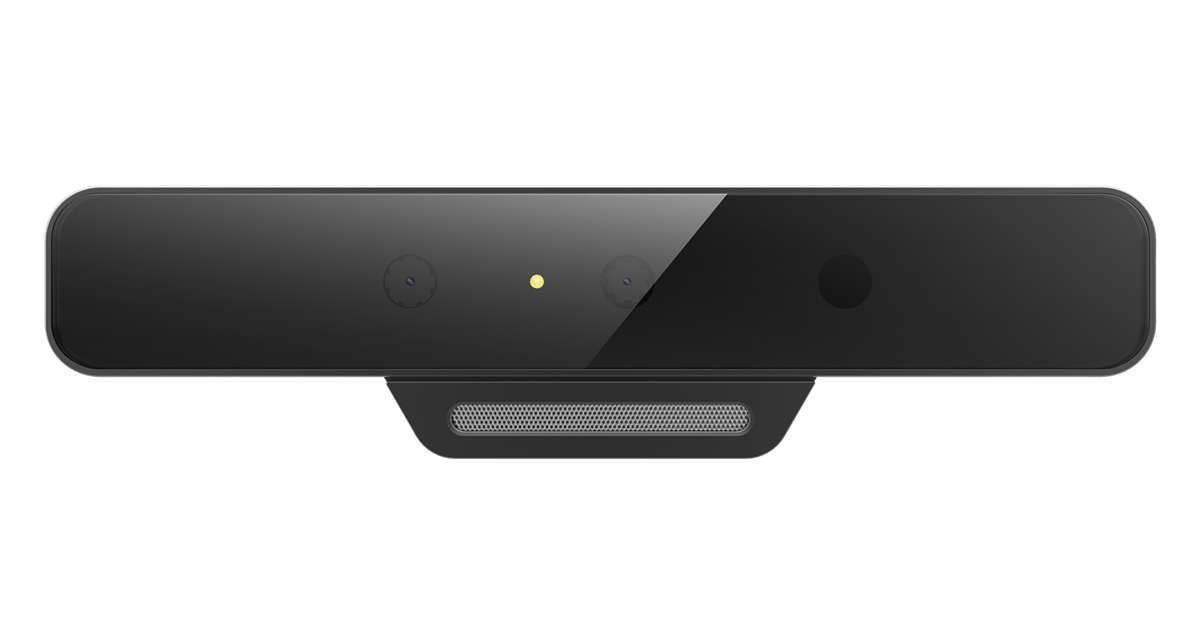
\includegraphics[width=0.4\textwidth]{rs_front.png}}
	\vspace{0.5cm}
	\caption{Внешний вид 3D-камеры Intel RealSense SR300}
	\label{img:camera}
\end{figure}

\begin{table}[h!]
	\centering\caption{Параметры инфракрасной и цветной камер RealSense~SR300}
	\label{table_gen_info_of_camera}
	\begin{tabularx}{\textwidth}{|Y|Y|Y|}
		\hline
		\multicolumn{1}{|c|}{Параметр} & ИК-камера                & RGB-камера               \\ \hline
		Разрешение, пикс               & $640 \times 480$         & $1920 \times 1080$       \\ \hline
		Вертикальный угол обзора, град   & $55 \pm 2$   & $41.5 \pm 2$ \\ \hline
		Горизонтальный угол обзора, град & $71.5 \pm 2$ & $68 \pm 2$   \\ \hline
		Диагональный угол обзора, град   & $88 \pm 3$   & $75.2 \pm 4$ \\ \hline
	\end{tabularx}
\end{table}

\begin{figure}[h!]
	\centering{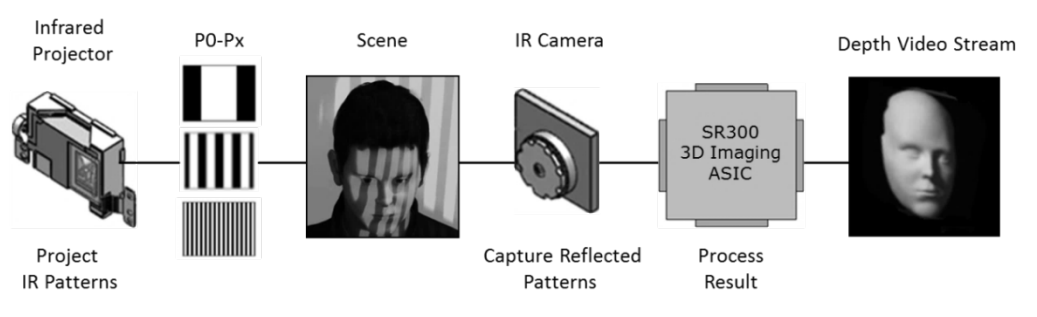
\includegraphics[width=0.9\textwidth]{sr300_depth.png}}
	\vspace{0.5cm}
	\caption{Принцип получения карты глубины}
	\label{img:camera2}
\end{figure}


\begin{table}[]
	\centering
	\caption{Параметры лазерного проектора камеры Intel~RealSense~SR300}
	\label{table_gen_info_of_camera2}
\begin{tabularx}{\textwidth}{|Y|Y|}
	\hline
	\multicolumn{1}{|c|}{Параметр} & Описание                                      \\ \hline
	Проектор                       & Структурированный свет                        \\ \hline
	Длина волны лазера, нм         & 860                                         \\ \hline
	Безопасность лазера            & Class 1                                       \\ \hline
	Вертикальный угол проекции, град     & $60 \pm 4$                        \\ \hline
	Горизонтальный угол проекции, град   & $72.5 \pm 2$ \\ \hline
\end{tabularx}
\end{table}

\subsection{Постановка и описание задачи}

Требуется оценить параметры траектории движения объекта покоящегося на вращающемся столе, пример которого представлен на рисунках~\ref{img:ws_and_conveyer.pdf}--\ref{img:trajectory_planning}. Траектория движения~--- окружность. Подлежащие оценке параметры: $ R_c $~--- радиус окружности, которую описывает объект при вращении стола, $ Oxyz $~--- СК вращающегося стола, где $Oz$~--- ось вращения, $ \bm{p}_0 $ и $ \bm{p_f} $~--- точки входа в нормальную рабочую область манипулятора и выхода из нее соответственно, а также векторы $ \bm{s}_o$ и $ \dot{\bm{s}}_o$~--- положение объекта в пространстве и скорость, выраженные в СК $ Ox_{0}y_{0}z_{0} $:
\begin{equation}
	\bm{s}_o =
	\begin{bmatrix}
		\bm{p}_o \\
		\bm{r}_o
	\end{bmatrix},
	\quad
	\dot{\bm{s}}_o =
	\begin{bmatrix}
		\bm{v}_o \\
		\bm{\omega}_o
	\end{bmatrix}\!\!.
\end{equation}
Объект представлен в лице прямоугольного параллелепипеда.

Выделим на вращающющемся столе две зоны: приближение объекта и захвата.
Тогда, сценарий работы СТЗ следующий:
\begin{enumerate}
	\item Манипулятор принимает конфигурацию, при которой в кадр камеры попадает зона приближения объекта;
	\item Проводится процедура выделения объекта из окружающей среды и  определение его геометрии, с последующим оцениванием векторов его положения $ \bm{s}_o $ и скорости $ \dot{\bm{s}}_o $;
	\item По собранной статистике о положении и ориентации объекта на столе за время $ \Delta t $, производится оценка оси вращения стола ${\overrightarrow{\bm{n}}}$ и радиуса кривизны траектории движения объекта $ R_c $.
	\item Перед тем, как закончить свою работу, СТЗ определяет точки входа $ \bm{p}_0 $ в зону захвата и выхода $ \bm{p}_f $ из нее объекта. После этого вся накопленная информация пересылается в генератор траекторий для манипулятора.
\end{enumerate}

Первый пункт рассматривается в разделе~\ref{part_kinematic_control}, последний в~\ref{part_trajectory}, а второй и третий реализуем в этом разделе. 

Прежде, чем приступить к решению поставленных задач, сделаем два замечания:
\begin{enumerate}
	\item Использование камеры Intel RealSense SR300 позволяет упростить решение поставленных задач, так как позволяет сразу работать с \textit{облаком точек}~--- набором вершин в трехмерном пространстве, координаты которых выражены в СК камеры; также, каждая точка может иметь цвет, например, в цветовой модели RGB;
	\item Работа с глубинными картами предполагает большой объем вычислений, поэтому необходим достаточно производительный компьютер.
\end{enumerate}

Непрерывно изменяющееся состояние окружающего мира~--- вращение стола, ~--- обязывает робототехническую систему работать в реальном времени, так как нет априорной информации о расположении объектов на нем. В связи с этим, необходимо найти компромисс между точностью работы системы и скоростью  вычислений обеспечивающих достаточную точность.

Как видно из таблицы~\ref{table_gen_info_of_camera}, разрешение получаемой карты глубины и, соответственно, облака точек равно $ 640 \times 480 $, что соответствует $ 307200$ точкам, представляющих из себя, в простейшем случае, структуру из трех координат положения точки и трех векторов, задающих ориентацию, т.е. в сумме, один кадр облака может содержать от четырехсот байт. При работе с частотой 30 кадров в секунду возрастает до двенадцати мегабайт. Дополнительным аргументом становится тот факт, что при уменьшении количества точек в облаке до некоторого порога, возможно добиться не худшей точности, чем при использовании всех точек. Из этих соображений имеет смысл понизить разрешение.

Среди огромного количества фильтров разной степени сложности, выберем наиболее простой, суть которого заключается в представлении облака точек в виде восьмиричного дерева~--- октодерева. Октодерево делит облако точек на октанты (воксели), каждый из которых рекурсивно делится до тех пор, пока каждая из точек не будет в отдельном октанте. Такое представление позволяет задавать разрешение облака точек простым изменением глубины октодерева~\cite{moreno2016comparative}. Пример деления представлен на рисунке~\ref{img:octree}.

\begin{figure}[h!]
	\centering{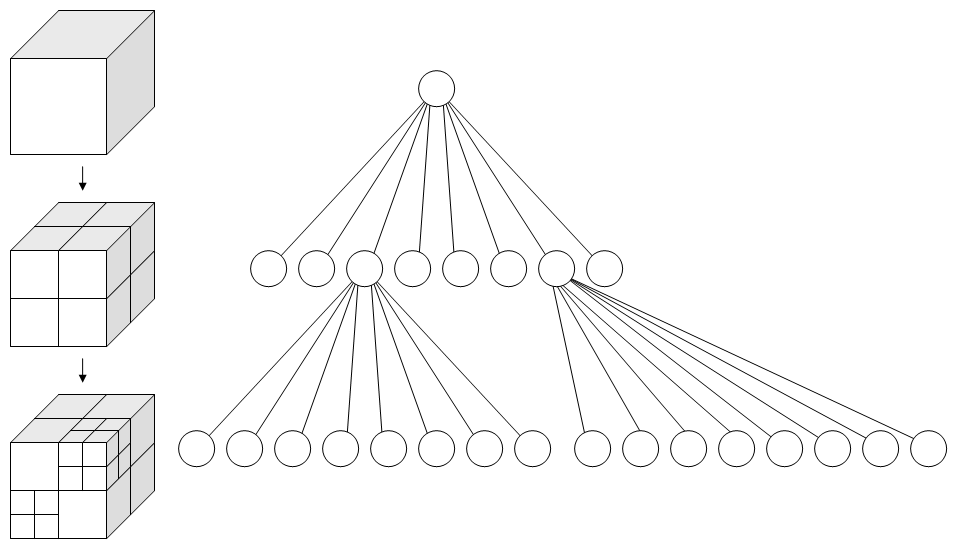
\includegraphics[width=0.7\textwidth]{octree.png}}
	\vspace{0.5cm}
	\caption{Изображение рекурсивного разделения куба на октанты и, соответствующее этому разделению, октодерево}
	\label{img:octree}
\end{figure}

Следующим этапом нужно определить плоскость вращающегося стола, на котором располагаются интересные нам объекты. Для этого воспользуемся методом оценки параметром плоскости на основе случайных выборок точек~--- RANSAC.

На вход алгоритма подается все облако точек, модель плоскости, которую нужно вписать в это болако, минимальное и максимальное число точек, которые могут входить в плоскость и максимальный разброс. На выходе получем параметры модели плоскости и точки, который входят в эту плоскость. На рисунке~\ref{img:plane} изображен пример результата работы. 

\begin{figure}[h!]
	\centering{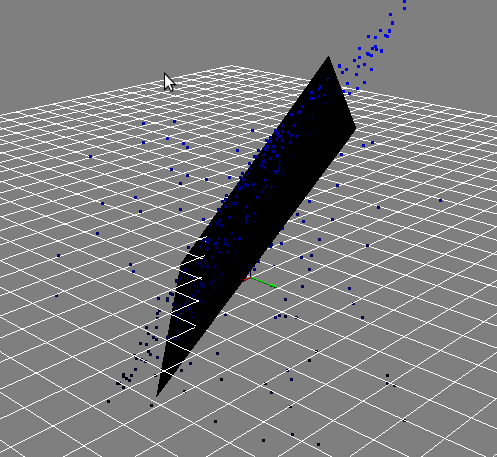
\includegraphics[width=0.7\textwidth]{plane.png}}
	\vspace{0.5cm}
	\caption{Пример вписывания плоскости в облако точек алгоритмом RANSAC}
	\label{img:plane}
\end{figure}

После определения кластера облака точек, в который входят все точки самой большой плоскости в кадре, то есть плоскости конвейера, необходимо найти объекта на этой плоскости. Для этого, построим выпуклую оболочку кластера облака точек входящих в плоскость, получив таким образом некоторый многоугольник. Далее, отбросив все точки, которе не входят в множество, включающее только внутреннюю часть призмы заданной высоты построенной на этом многоугольнике, получим все объекты расположенные на столе. В этой работе рассматривается только один объект, но это решение легко можно расширить на большее их число путем деление кластера с объектами на еще более мелкие кластеры, содержание каждый свой объект~\cite{toold3dthesis}.

Теперь, имея облако точек, включающее только целевой объект, необходимо найти его центр масс и ориентацию. Для этого воспользуемся методом определения момента инерции облака точек. Идея метода заключается в следующем. Вычисляется ковариационная матрица точечного облака и извлекаются ее собственные значения и векторы, которые представляют собой оси x, y и z, образующие ортогональный правый базис. На каждой итерации выбирается один из полученных векторов, причем вращение всегда одинаковое, что обеспечивает инвариантность к вращению всего рассматриваемого облака точек. После этого, для каждой оси рассчитывается момент инерции.

Полученные значения поворота облака точек и его центр масс будем использовать для оценки траектории движения объекта. Причем, ориентацию объекта достаточно оценить один раз, а после задавать ее дополнительное слагаемое к углу поворота вращающегося стола.

Последним этапом работы технического зрения является отслеживание траектории движения объекта и одновременная идентификация параметров этой траектории заданной в параметрической форме окружности:
\begin{equation}
\begin{cases}
	x(t) = R_c \cos{\theta(t)}\\
	y(t) = R_c \sin{\theta(t)} \\
	z(t) = const
\end{cases}\!\!\!\!\!\!\!\!,
\end{equation}
где $ R_c $~--- радиус окружности, описываемой объектом при вращении стола, $ \theta(t) $~--- поворот стола.

Таким образом, нужно найти радиус дуги, которую описывает объект при вращении стола.
Рассмотрим случай нахождения радиуса по трем известным координатам точек окружности $ A(x_1,y_1),\: B(x_2, y_2) $ и $ C(x_3, y_4) $. Возможный пример такого случая изображен на рисунке~\ref{img:circle} 

\begin{figure}[h!]
	\centering{\includegraphics[width=0.7\textwidth]{ipe/circle.pdf}}
	\vspace{0.5cm}
	\caption{Нахождение радиуса окружности по известным точкам, пренадлежащим окружности}
	\label{img:circle}
\end{figure}

Запишем уравнения для прямых $ a $ и $ b $:

\begin{gather}
	y_a = k_a (x - x_1) + y_1, \quad y_b = k_b (x - x_2) + y_2,
\end{gather}
где $ k_a$~--- коэффициент наклона прямой a, $ k_b $~--- коэффициент наклона прямой~b.

Коэффициенты рассчитываются из следующих соотношений:
\begin{equation}
	k_a = \cfrac{y_2 - y_1}{x_2 - x_1}, \quad k_b = \cfrac{y_3 - y_2}{x_3 - x_2}.
\end{equation}

Далее, найдем центр окружности, который находится на пересечении прямых проведенных через середины отрезков AB и BC. Учитывая, что коэффициент наклона перпендикулярна выражается как $ k_{a,b} = -\frac{1}{m_{a,b}}  $, запишем уравнения перпендикуляров:
\begin{equation}
	y_{\perp a} = - \cfrac{1}{k_a} \cdot \Bigg( x - \cfrac{x_1 + x_2}{2}\Bigg) + \cfrac{y_1 + y_2}{2}, \quad
	y_{\perp b} = - \cfrac{1}{k_b} \cdot \Bigg( x - \cfrac{x_2 + x_3}{2}\Bigg) + \cfrac{y_2 + y_3}{2}.
\end{equation}

И, так как полученные перпендикуляры пересекаются ровно в центре окружности, запишем для координат точки O:
\begin{gather}
	x = \cfrac{k_a k_b ( y_1 - y_3) + k_b (x1 + x2) - k_a (x_2 + x3)}{2 (k_b - k_a)},
\end{gather}
\begin{align*} 
	y = - \cfrac{1}{k_a} \cdot \Bigg( \cfrac{k_a k_b ( y_1 - y_3) + k_b (x1 + x2) - k_a (x_2 + x3)}{2 (k_b - k_a)} -\\- \cfrac{x_1 + x_2}{2} \Bigg) + \cfrac{y_1 + y_2}{2}.
\end{align*}

Имея оценку координат центра окружности, по которой двигается объект, легко найти радиус:
\begin{equation}
	R_c = \sqrt{(x - x_3)^2 + (y - y_3)^2}
\end{equation}

Таким образом, при слежении за объектом в области перед точкой $ P_0 $ для каждой полученной последовательности трех точек рассчитывается оценка радиусу. Со временем накапливаются возможные значения радиусов и координат его центра. Координаты центра следует отфильтровать, найдя центр минимальной окружности, которая охватывает большинство точек оценок координат центра траектории движения объекта.

Описанная последовательность действий позволяет определить положение и ориентацию объекта на вращающемся столе, а также момент входа объекта в область доступную для захватывания его манипулятором.

